\documentclass[nonatbib]{article}


% if you need to pass options to natbib, use, e.g.:
%     \PassOptionsToPackage{numbers, compress}{natbib}
% before loading neurips_2022


% ready for submission
\usepackage{neurips_2022}


% to compile a preprint version, e.g., for submission to arXiv, add add the
% [preprint] option:
%     \usepackage[preprint]{neurips_2022}


% to compile a camera-ready version, add the [final] option, e.g.:
%     \usepackage[final]{neurips_2022}


% to avoid loading the natbib package, add option nonatbib:
%    \usepackage[nonatbib]{neurips_2022}


\usepackage[utf8]{inputenc} % allow utf-8 input
\usepackage[T1]{fontenc}    % use 8-bit T1 fonts
\usepackage{hyperref}       % hyperlinks
\usepackage{url}            % simple URL typesetting
\usepackage{booktabs}       % professional-quality tables
\usepackage{amsfonts}       % blackboard math symbols
\usepackage{nicefrac}       % compact symbols for 1/2, etc.
\usepackage{microtype}      % microtypography
\usepackage{xcolor}         % colors

\usepackage{graphicx}
%Custom comments
%Commands & Other packages
\usepackage{wrapfig}
\usepackage{slashbox}
\newcommand{\indep}{\perp \!\!\! \perp}
\newcommand{\indepnot}{\not\!\perp\!\!\!\perp}
\newcommand{\E}{\mathbb{E}}
\newcommand{\R}{\mathbb{R}}
\newcommand{\N}{\mathbb{N}}
\newcommand{\TODO}[1]{{\color{red}#1}}
\newcommand{\makeblue}[1]{{\color{blue}#1}}
\newcommand{\makered}[1]{{\color{red}#1}}
\usepackage{xspace}
  \newcommand{\eg}{e.\,g.\xspace}
  \newcommand{\ie}{i.\,e.\xspace}
\usepackage{enumitem}
\usepackage{bbm}
\usepackage{setspace}
\makeatletter
\newcommand{\settitle}{\@maketitle}
\makeatother
\newcommand{\frameworkname}{MRIV\xspace}
\newcommand{\modelname}{\mbox{MRIV-Net}\xspace}

%Theorems % Algorithms
\usepackage{amssymb,amsmath,amsthm}
\usepackage{algorithm2e}
\RestyleAlgo{ruled}
\theoremstyle{definition}
\newtheorem{assumption}{Assumption}
\theoremstyle{plain}
\newtheorem{lemma}{Lemma}
\newtheorem{theorem}{Theorem}
\newtheorem{corollary}{Corollary}

%bibliography
\usepackage[backend=biber, style=numeric, doi=false, isbn=false, url=false, eprint=false]{biblatex}
\addbibresource{bibliography.bib}


\title{Estimating individual treatment effects under unobserved confounding using binary instruments}


% The \author macro works with any number of authors. There are two commands
% used to separate the names and addresses of multiple authors: \And and \AND.
%
% Using \And between authors leaves it to LaTeX to determine where to break the
% lines. Using \AND forces a line break at that point. So, if LaTeX puts 3 of 4
% authors names on the first line, and the last on the second line, try using
% \AND instead of \And before the third author name.


\author{%
  Dennis Frauen \\
  LMU Munich\\
  \texttt{frauen@lmu.de} \\
  % examples of more authors
  \And
  Stefan Feuerriegel \\
  LMU Munich \\
  \texttt{feuerriegel@lmu.de}
}


\begin{document}


\settitle

\begin{abstract}
Estimating individual treatment effects (ITEs) from observational data is relevant in many fields such as personalized medicine. However, in practice, the treatment assignment is usually confounded by unobserved variables and thus introduces bias. A remedy to remove the bias is the use of instrumental variables (IVs). Such settings are widespread in medicine (e.g., trials where compliance is used as binary IV). In this paper, we propose a novel, multiple robust machine learning framework, called \frameworkname, for estimating ITEs using binary IVs and thus yield an unbiased ITE estimator. Different from previous work for binary IVs, our framework estimates the ITE directly via a pseudo outcome regression. (1)~We provide a theoretical analysis where we show that our framework yields multiple robust convergence rates: our ITE estimator achieves fast convergence even if several nuisance estimators converge slowly. (2)~We further show that our framework asymptotically outperforms state-of-the-art plug-in IV methods for ITE estimation. (3)~We build upon our theoretical results and propose a tailored deep neural network architecture called \modelname for ITE estimation using binary IVs. Across various computational experiments, we demonstrate empirically that our \modelname achieves state-of-the-art performance. To the best of our knowledge, our \frameworkname is the first multiple robust machine learning framework tailored to estimating ITEs in the binary IV setting. 
\end{abstract}


\section{Introduction}

%(individual) Causal effects, observational data, confounding

Individual treatment effects (ITEs) are relevant across many disciplines such as personalized medicine \cite{Yazdani.2015} or marketing \cite{Varian.2016}. Knowledge about ITEs can be helpful to assign treatments to individuals that maximize their benefit. For instance, the effect of a medicament on a patients probability of survival might depend on various factors such as age, and the treatment might only be helpful for older patients. Due to the increasing amounts of observational data, recent work has focused on using machine learning to estimate ITEs \cite{Shalit.2017, Alaa.2017, Yoon.2018}. However, estimating ITEs from observational data is challenging \cite{Alaa.2018}. This is because the treatment alignment mechanism underlying observational data is confounded with the outcome. In order to produce unbiased estimates, many modern methods assume that all confounders are reported in the data.

% Instrumental variables 

In practice however, it is common that unobserved confounders exist. Hence, standard methods for estimating ITEs suffer from confounding bias \cite{Pearl.2009}. As a remedy, instrumental variables (IVs) can be leveraged if available to construct methods that provide more reliable ITE estimates. IV methods were originally used in econonmics \cite{Wright.1928}, but have also been applied in other fields. They relax the assumption of no unobserved confounding, but require additional assumptions on the instruments. For example, the instruments are not allowed to have a direct causal effect on the outcome of interest, but they need to be correlated with the treatment variable. If these assumptions are met, IV methods outperform classical ITE estimators if a sufficient amount of confounding is not observed \cite{Hartford.2017}.

% Our setting - non-compliance

In this paper, we consider the setting where a single binary instrument is available. This is particularly relevant in observational or randomized studies with observed non-compliance \cite{Imbens.1994}. As an example, consider a randomized controlled trial, where treatments are randomly assigned to patients and their outcomes are observed. Due to some potentially unobserved confounders (e.g., health conditions), some patients refuse to take the treatment initially assigned to them. Here, the treatment assignment can be used as an IV to estimate the causal effect of the treatment on the outcome. Most IV assumptions are automatically satisfied because the treatment assignment affects the outcome only via the actual treatment. 

\TODO{move} This is in contrast to more general IV settings, where IV assumptions can be controversial in practice \cite{Wooldridge.2013}.

%Method

We propose a multiple robust machine learning framework for estimating ITEs using binary IVs. We call our framework \frameworkname. Importantly, our framework is multiple robust, i.e., it is consistent even if several inputs are misspecified. Existing methods aimed at binary IVs are plug-in estimators \TODO{REf}. These are not multiple robust and, on top of that, it is well known that such estimators suffer from plug-in bias \TODO{REF}. To address this, our key innovation is: Different from existing works, we estimate the ITE directly by performing a pseudo outcome regression on a multiple robust parametrization of the efficient influence function. As such, we refrain from estimating the different components of the ITE individually but, instead, leverage the pseudo outcome. 

We provide a theoretical analysis where we show that our framework achieves a multiple robust convergence rate, i.e., our \frameworkname converges with a fast rate even if several nuisance parameters converge slowly. We further show that, compared to existing plug-in IV methods, the performance of our framework is asymptotically superior. Finally, we leverage our framework to integrate it into a tailored deep neural network called \modelname. We perform computational experiments using simulated and real-world medical data to demonstrate that our \modelname has a superior performance compared to existing methods by a large margin. 


% \frameworkname is motivated by the idea to remove plug-in bias via influence functions \cite{Curth.2020}. Given an initial ITE estimate, \frameworkname performs a regression on a pseudo outcome that resembles a multiple robust parametrization of the uncentered influence function for the \emph{average} treatment effect \cite{Wang.2018}. By doing so, \frameworkname achieves a multiple robust rate of convergence, meaning that the corresponding ITE estimator converges fast even if several nuisance estimators or the initial estimator converge slowly. Furthermore, \frameworkname omits estimating the different components of the ITE individually, leading to superior performance if the true ITE curve is easier to estimate than its components, which is usually the case in practice \cite{Kunzel.2019}. We confirm this intuition both theoretically and empirically, by comparing \frameworkname to several other IV methods. Finally, we propose a tailored deep neural network, called \modelname. Our \modelname uses two separate shared representations to estimate the initial components of \frameworkname. In our experiments, we compare the performance of \frameworkname for several initial estimators and show that \modelname is state-of-the-art.

% Furthermore, \frameworkname omits estimating the different components of the ITE individually, leading to superior performance if the true ITE curve is easier to estimate than its components, which is usually the case in practice \cite{Kunzel.2019}.
% Previous methods tailored to the binary IV setting are plug-in estimators, and it is well known that such estimators suffer from plug-in bias. \frameworkname is motivated by the idea to remove plug-in bias via influence functions \cite{Curth.2020}. Given an initial ITE estimate, \frameworkname performs a regression on a pseudo outcome that resembles a multiple robust parametrization of the uncentered influence function for the \emph{average} treatment effect \cite{Wang.2018}.

\textbf{Contributions:}\footnote{Codes are in the supplementary materials. Codes are also available at \href{https://anonymous.4open.science/r/MRIV-Net-0AC4}{https://anonymous.4open.science/r/MRIV-Net-0AC4} (Upon acceptance, we replace the link and point to a public GitHub repository).} (1)~We propose a novel, multiple robust machine learning framework (called \frameworkname) to learn the ITE using the binary IV setting. To the best of our knowledge, ours is the first that is multiple robust, i.e., consistent even if several inputs are misspecified. (2)~We prove that \frameworkname achieves a multiple robust convergence rate. We further show that our \frameworkname is asymptotically superior to existing plug-in estimators. (3)~We propose a tailored deep neural network, called \modelname, which builds upon our framework to estimate ITEs. We demonstrate that it achieves state-of-the-art performance.

% We show that our framework is multiple robust, i.e., consistent even if several inputs are misspecified.

\section{Problem setup}

\begin{wrapfigure}{r}{0.3\textwidth}
\vspace{-2cm}
\begin{center}
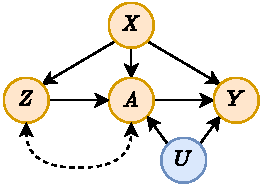
\includegraphics[width=0.3\textwidth]{img/causal_graph.pdf}
\end{center}
\caption{Underlying causal graph. The instrument $Z$ has a direct influence on the treatment $A$, but does not have a direct effect on the outcome $Y$. Note that we allow for unobserved confounders for both $Z$--$A$ (dashed line) and $A$--$Y$ (given by $U$).}
\label{fig:causal_graph}
\vspace{-0.5cm}
\end{wrapfigure}

\textbf{Data generating process:}
We observe data $\mathcal{D} = (x_i, z_i, a_i, y_i)_{i=1}^n$ consisting of $n \in \N$ observations of the tuple $(X, Z, A, Y)$.
Here, $X \in \mathcal{X}$ are observed confounders, $Z \in \{0, 1\}$ is a binary instrument, $A \in \{0, 1\}$ is a binary treatment, and $Y \in \R$ is an outcome of interest. Furthermore, we assume the existence of unobserved confounders $U \in \mathcal{U}$, which affect both the treatment $A$ and the outcome $Y$. The causal graph is shown in Fig.~\ref{fig:causal_graph}.

The above setting is widespread in practice, e.g., in personalized medicine. It is particularly relevant when individuals do not comply with their treatment assignment. For instance, it has been widely used for randomized controlled trials (RCT) with non-compliance, e.g., to study the effect of health insurance on health outcome \cite{Finkelstein.2012} or the effect of military service on lifetime earnings \cite{Angrist.1990}. In this case, the instrument $Z$ is the treatment assignment and indicates the decision whether a patient should receive treatment. Note that modeling treatments as binary variables is consistent with previous literature on causal effect estimation and standard in medical practice \cite{Robins.2000}. 

We build upon the potential outcomes framework \cite{Rubin.1974} for modeling causal effects. Let $Y(a,z)$ denote the potential outcome that would have been observed under $A=a$ and $Z=z$. Following previous literature on IV estimation \cite{Wang.2018}, we impose the following standard IV assumptions on the data generating process.

\begin{assumption}[Standard IV assumptions]
\label{ass:iv}
We assume: (1)~\emph{Exclusion:} $Y(a,z) = Y(a)$ for all $a, z \in \{0,1\}$, i.e., the instrument has no direct effect on the patient outcome; (2)~\emph{Independence:} $Z \indep U \mid X$; (3)~\emph{Relevance:} $Z \indepnot A \mid X$, (iv)~\emph{The model includes all $A$--$Y$ confounder:} $Y(a) \indep (A, Z) \mid (X, U)$ for all $a \in \{0,1\}$.
\end{assumption}

Assumption 1 is fairly unrestrictive an widespread in practice \cite{Angrist.1990, Angrist.1991, Imbens.1994}. Note that Assumption~\ref{ass:iv} does not prohibit the existence of unobserved $Z$--$A$ confounders. On the contrary, it merely prohibits the existence of unobserved counfounders that affect all $Z$, $A$, and $Y$, simultaneously, as it is standard in IV settings \cite{Wooldridge.2013}. A practical and widespread example where Assumption~\ref{ass:iv} is satisfied are randomized controlled trials~(RCTs) with non-compliance \cite{Imbens.1994}. Here, the treatment assignment $Z$ is randomized, but the actual relationship between treatment $A$ and outcome $Y$ may still be confounded. For instance, in the \emph{Oregon health insurance experiment} \cite{Finkelstein.2012}, people were given access to health insurance ($Z$) by a lottery, in hope to study the effect of health insurance ($A$) on health outcome ($Y$) \cite{Finkelstein.2012}. Here, non-compliance information is observed because the lottery winners needed to sign up for health insurance.

\textbf{Objective:} 
In this paper, we are interested in estimating the \emph{individual treatment effect} (ITE)
\begin{equation}
  \tau(x) = \E[Y(1) - Y(0) \mid X = x].
\end{equation}
If there is no unobserved confounding ($U = \emptyset$), the ITE is identifiable from observational data under mild positivity assumptions \cite{Shalit.2017}. However, in practice, it is often unlikely that all confounders are observable. To account for this, we leverage the instrument $Z$ to identify the ITE. We state the following assumption for identifiability.

\begin{assumption}[Identifiability of the ITE]\label{ass:identification}
    At least one of the following two statements holds true: (1)~There is no additive $U$--$Z$ interaction in $\E[A \mid Z, X, U]$, i.e.,
    \begin{equation}
    \E[A \mid Z=1, X, U] - \E[A \mid Z=0, X, U] = \E[A \mid Z=1, X] - \E[A \mid Z=0, X];
    \end{equation}   
    or (2)~there is no additive $U$--$a$ interaction in $\E[Y(a) \mid X, U]$, i.e.,
    \begin{equation}
    \E[Y(1) - Y(0) \mid X, U] = \E[Y(1) - Y(0) \mid X].    
    \end{equation}
\end{assumption}

Under Assumptions \ref{ass:iv} and \ref{ass:identification}, the ITE is identifiable \cite{Wang.2018}. It can be written as
\begin{equation}
\label{eq:identification}
    \tau(x) = \frac{\mu_1^Y(x) - \mu_0^Y(x)}{\mu_1^A(x) - \mu_0^A(x)} = \frac{\delta_Y(x)}{\delta_A(x)},
\end{equation}
where $\mu_i^Y(x) = \E[Y \mid Z = i, X = x]$ and $\mu_i^A(x) = \E[A \mid Z = i, X = x]$. Even if Assumption~\ref{ass:identification} does not hold, the quantity on the right-hand side of Eq.~\eqref{eq:identification} still allows for interpretation. If no unobserved $Z$--$A$ confounders exist, it can be interpreted as conditional version of the \emph{local average treatment effect}~(LATE) \cite{Imbens.1994, BargagliStoffi.2021} under a monotonicity assumption. Furthermore, under a no-current-treatment-value-interaction assumption, it can be interpreted as conditional \emph{treatment effect on the treated}~(ETT) \cite{Wang.2018}. \footnote{The conditional LATE measures the ITE for individuals which are part of the complier subpopulation, i.e., the subpopulation for which it holds that $Z = A$. The conditional ETT measures the ITE for treated individuals.} This has an important implication for our results: If Assumption~\ref{ass:identification} does not hold in practice, our estimates still provide conditional LATE or ETT estimates under the respective assumptions because they build on Eq.~\eqref{eq:identification}. If Assumption~\ref{ass:identification} does hold, all ITE, conditional LATE, and ETT coincide \cite{Wang.2018}.

\section{Related work}

\textbf{ITE methods without unconfoundedness:} Various machine learning methods for estimating ITEs \emph{without} unobserved confounding have been proposed in recent literature. Examples include tree-based methods \cite{Wager.2018}, Bayesian nonparametric methods \cite{Alaa.2017}, and deep neural networks \cite{Shalit.2017, Yoon.2018, Zhang.2020}. Other works have developed meta-learners \cite{Kunzel.2019}, which have also been instantiated with deep neural networks \cite{Curth.2021}. To remove plug in bias, the DR learner performs a second stage regression on the uncentered influence function of the average treatment effect \cite{Kennedy.2020, Curth.2020}. However, under unobserved confounding, all of these methods are biased (see Appendix\TODO{Ref}). As a result, this hampers their performance in our setting. 

%In a related stream, methods for deconfounding have been proposed, which exploit correlations between multiple \cite{Wang.2019} or time-varying treatments \cite{Bica.2020b, Hatt.2021b}. However, these are not applicable in our setting.

\textbf{ITE methods for unobserved confounding:}
IV methods address the problem of unobserved confounding by exploiting the variance in treatment and outcome induced by the instruments. Traditionally, two-stage least squares (2SLS) has been used for estimating causal effects \cite{Wright.1928, Angrist.1991}. 2SLS was originally developed in economics, and follows a two-stage procedure: it performs a first stage regression of treatment $A$ on the instrument $Z$, and then uses the fitted values for a second stage regression to predict the outcome $Y$. Several nonparametric methods have been developed in econometric to generalize 2SLS in order to account for non-linearities within the data \cite{Newey.2003, Wang.2021}, yet these are limited to low-dimensional settings.

Only recently, machine learning has been integrated into IV methods. These are: Kernel~IV \cite{Singh.2019} and DFIV \cite{Xu.2021} generalize 2SLS by learning complex feature maps using kernel methods and deep learning, respectively. DeepIV \cite{Hartford.2017} adopts a two-stage neural network architecture that performs the first stage via conditional density estimation. DeepGMM \cite{Bennett.2019} and DMLIV \cite{Syrgkanis.2019} leverage moment conditions for IV estimation. Finally, DRIV \cite{Syrgkanis.2019} is a doubly robust machine learning framework to estimate ITEs via a pseudo outcome regression. However, all methods mentioned are not specifically designed for the binary IV setting but, rather, for multiple IV or treatment scenarios. Hence, they require additive confounding in order to identify the ITE. We show in our experiments that, even under additive confounding, our framework outperforms the above IV methods.

\textbf{Binary IVs:} In the binary IV setting, current methods proceed by estimating $\mu_i^Y(x)$ and $\mu_i^A(x)$ separately, before  plugging them in Eq.~\ref{eq:identification} \cite{Imbens.1994, Angrist.1996, BargagliStoffi.2021}. As result, these suffer from plugin bias and do \emph{not} enjoy robustness properties. In contrast, multiple robust estimators based on semiparametric efficiency theory have been proposed only for average treatment effects (ATEs) and \underline{not} for ITEs. For example, for ATEs, \cite{Wang.2018} derive a multiple robust parametrization of the efficient influence curve for the uncentered ATE in the binary setting. However, there exists no similar approach for ITE estimation.

\textbf{Research gap:} To the best of our knowledge, there exists no method for ITE estimation under unobserved confounding that is multiple robust. As a remedy, we propose \frameworkname, a multiple robust machine learning framework tailored to the binary IV setting.


\section{\frameworkname for estimating ITEs using binary instruments}

In the following, we present our \frameworkname framework for estimating ITEs under unobserved confounding (Sec.~\ref{sec:methodology}). We then derive we derive an asymptotic convergence rates for \frameworkname (Sec.~\ref{sec:theory}) and finally use our framework to develop a tailored deep neural network called \modelname (Sec.~\ref{sec:neural_nets}). 

\subsection{Framework}
\label{sec:methodology}

\TODO{DISCUSS: Previous methods tailored to the binary IV setting are plug-in estimators, and it is well known that such estimators suffer from plug-in bias. \frameworkname is motivated by the idea to remove plug-in bias via influence functions \cite{Curth.2020}. Given an initial ITE estimate, \frameworkname performs a regression on a pseudo outcome that resembles a multiple robust parametrization of the uncentered influence function for the \emph{average} treatment effect \cite{Wang.2018}.}

\textbf{Motivation:} A na{\"i}ve approach to estimate the ITE is to leverage the identification result in Eq.~\eqref{eq:identification}. Assuming that we have estimated the ITE components $\hat{\mu}_i^Y$ and $\hat{\mu}_i^A$ for $i \in \{0,1\}$, the (plug-in) Wald estimator \cite{Wald.1940} is then defined as
\begin{equation}\label{eq:wald}
    \hat{\tau}_{\mathrm{W}}(x) = \frac{\hat{\mu}_1^Y(x) - \hat{\mu}_0^Y(x)}{\hat{\mu}_1^A(x) - \hat{\mu}_0^A(x)}.
\end{equation}
However, in practice, the true ITE curve $\tau(x)$ is often simpler (e.g., smoother, more sparse) than its complements $\mu_i^Y(x)$ or $\mu_i^A(x)$ \cite{Kunzel.2019}. In this case, $\hat{\tau}_{\mathrm{W}}(x)$ is inefficient because it models all components separately.

\textbf{Overview:} We now propose \frameworkname.  \frameworkname is a two-stage meta learner that takes any base method for ITE estimation as input. For instance, the base method could be the Wald estimator from Eq.~\eqref{eq:wald} or any other IV method such as 2SLS. In Stage 1, \frameworkname produces nuisance estimators $\hat{\mu}_0^Y(x)$, $\hat{\mu}_0^A(x)$, $\hat{\delta}_A(x)$, and $\hat{\pi}(x)$, where $\hat{\pi}(x)$ is an estimator of the propensity score $\pi(x) = \mathbb{P}(Z = 1 \mid X = x)$. In Stage 2, \frameworkname directly estimates $\tau(x)$ by using a pseudo outcome $\hat{Y}_0$ as a  regression target. 

Given an arbitrary initial ITE estimator $\hat{\tau}_{\mathrm{init}}(x)$ and nuisance estimates $\hat{\mu}_0^Y(x)$, $\hat{\mu}_0^A(x)$, $\hat{\delta}_A(x)$, and $\hat{\pi}(x)$, we define the pseudo outcome
\begin{equation}
\label{eq:pseudo_outcome}
    \hat{Y}_0 = \left(\frac{Z -(1-Z)}{\hat{\delta}_A(X)}\right) \left( \frac{Y - A \, \hat{\tau}_{\mathrm{init}}(X) - \hat{\mu}_0^Y(X) + \hat{\mu}_0^A(X) \, \hat{\tau}_{\mathrm{init}}(X)}{Z \, \hat{\pi}(X) + (1-Z) (1-\hat{\pi}(X))}\right) + \hat{\tau}_{\mathrm{init}}(X).
\end{equation}

Once we have obtained the pseudo outcome $\hat{Y}_0$, we regress it on $X$ to obtain the Stage 2 \frameworkname estimator $\hat{\tau}_{\mathrm{\frameworkname}}(x)$ for $\tau(x)$. The pseudocode for \frameworkname is given in Algorithm~\ref{alg:mr}.


\begin{algorithm}[H]
\DontPrintSemicolon
\caption{\frameworkname}
\label{alg:mr}
\footnotesize
        \SetKwInOut{Input}{Input}
\Input{~data $(X, Z, A, Y)$, initial ITE estimator $\hat{\tau}_{\mathrm{init}}(x)$}
\tcp{Stage 1: Estimate nuisance components}
$\hat{\pi}(x) \gets \hat{\E}[Z \mid X = x] $, \quad $\hat{\mu}_0^Y(x) \gets \hat{\E}[Y \mid X = x, Z = 0]$, \quad  $\hat{\mu}_0^A(x) \gets \hat{\E}[A \mid X = x, Z = 0]$\;
$\hat{\delta}_A(x) \gets \hat{\E}[A \mid X = x, Z = 1] - \hat{\E}[A \mid X = x, Z = 0]$\;
\tcp{Stage 2: Pseudo outcome regression}
$\hat{Y}_0 \gets \left( \frac{Z -(1-Z)}{\hat{\delta}_A(X)} \right) \left(\frac{Y - A \, \hat{\tau}_{\mathrm{init}}(X) - \hat{\mu}_0^Y(X) + \hat{\mu}_0^A(X) \, \hat{\tau}_{\mathrm{init}}(X)}{Z \, \hat{\pi}(X) + (1-Z) (1-\hat{\pi}(X))} \right) +\hat{\tau}_{\mathrm{init}}(X)$\;
$\hat{\tau}_{\mathrm{MRIV}}(x) \gets \hat{\E}[\hat{Y}_0 \mid X = x] $
\end{algorithm}

The pseudo outcome $\hat{Y}_0$ in Eq.~\eqref{eq:pseudo_outcome} is a multiple robust parameterization of the (uncentered) efficient influence curve for the average treatment effect $\E_X[\tau(X)]$ (see the derivation in \cite{Wang.2018}). Hence, \frameworkname can be interpreted as a way to remove plug-in bias from $\hat{\tau}_{\mathrm{W}}(x)$ via influence functions \cite{Curth.2020}. Using this observation, we derive the multiple robustness property of $\hat{\tau}_{\mathrm{MRIV}}(x)$ in Theorem~\ref{thrm:robustness}.

\begin{theorem}[Multiple robustness property]\label{thrm:robustness}
Let $\hat{\mu}_0^Y(x)$, $\hat{\mu}_0^A(x)$, $\hat{\delta}_A(x)$, $\hat{\pi}(x)$, and $\hat{\tau}_{\mathrm{init}}(x)$ denote estimators of $\mu_0^Y(x)$, $\mu_0^A(x)$, $\delta_A(x)$, $\pi(x)$, and $\tau(x)$, respectively. Then, for all $x \in \mathcal{X}$, it holds that $\E[\hat{Y}_0 \mid X = x] = \tau(x)$,if least one of the following conditions is satisfied:
\begin{enumerate}
    \item $\hat{\mu}_0^Y = \mu_0^Y$, $\hat{\mu}_0^A = \mu_0^A$, $\hat{\delta}_A = \delta_A$, and $\hat{\tau}_{\mathrm{init}} = \tau$; or
    \item $\hat{\pi} = \pi$ and $\hat{\delta}_A = \delta_A$; or
    \item $\hat{\pi} = \pi$ and $\hat{\tau}_{\mathrm{init}} = \tau$.
\end{enumerate}
\end{theorem}
Theorem~\ref{thrm:robustness} implies that $\hat{\tau}_{\mathrm{MRIV}}(x)$ is consistent for $\tau(x)$ even if several nuisance components are misspecified. It is consistent even when the initial ITE estimator $\hat{\tau}_{\mathrm{init}}$ is misspecified as long as the propensity estimator $\hat{\pi}(x)$ and $\hat{\delta}_A(x)$ are correctly specified.

%\textbf{Special case: RCT with non-compliance:} 
Our \frameworkname is directly applicable to RCTs with non-compliance. Then, the treatment assignment is randomized and the propoensity score $\pi(x)$ is known. Our \frameworkname framework can be then adopted by plugging in the known $\pi(x)$ into the pseudo outcome in Eq.~\eqref{eq:pseudo_outcome}. In this case $\hat{\tau}_{\mathrm{MRIV}}(x)$ is already consistent if either $\hat{\tau}_{\mathrm{init}}$(x) or $\hat{\delta}_A(x)$ are.

\subsection{Theoretical analysis}
\label{sec:theory}

In the following, we derive the asymptotic convergence rate of \frameworkname under smoothness assumptions. For this, we define $s$-smooth functions as functions contained in the Hölder class $\mathcal{H}(s)$, associated with Stone's minimax rate \cite{Stone.1980} of $n^{-2s/(2s+p)}$, where $p$ is the dimension of $\mathcal{X}$.

\begin{assumption}[Smoothness]\label{ass:smoothness}
We assume that (1)~the nuisance components $\mu_i^Y(\cdot)$ are $\alpha$-smooth, $\mu_i^A(\cdot)$ and $\delta_A(\cdot)$ are $\beta$-smooth, and $\pi(\cdot)$ is $\delta$-smooth; (2)~all nuisance components are estimated with their respective minimax rate of $n^{\frac{-2k}{2k+p}}$, where $k \in \{\alpha, \beta, \delta\}$; and (3)~the oracle ITE $\tau(\cdot)$ is $\gamma$-smooth and the initial ITE estimator $\hat{\tau}_{\mathrm{init}}$ converges with rate $r_{\tau}(n)$.
\end{assumption}

Assumption~\ref{ass:smoothness} for smoothness provides us with a way to quantify the difficulty of the underlying nonparametric regression problems. Similar assumptions have been imposed for asymptotic analysis of previous ITE estimators in \cite{Kennedy.2020, Curth.2021}. They can be replaced with other assumptions such as assumptions on the level of sparsity of the ITE components. We also provide an asymptotic analysis under sparsity assumptions, in Appendix~\ref*{app:sparsity}. 

We additionally impose the following boundedness assumptions on the the underlying data generating process and estimators.

\begin{assumption}[Boundedness]\label{ass:boundedness}
We assume that:
\begin{enumerate}
    \item $|\mu_i^Y(x)| \leq C$ for all $x \in \mathcal{X}$ and some constant $C>0$;
    \item $|\delta_A (x)| = |\mu_1^A(x) - \mu_0^A(x)| \geq \rho$ and $|\hat{\delta}_A (x)| \geq \widetilde{\rho}$ for all $x \in \mathcal{X}$ and constants $\rho, \widetilde{\rho}>0$;
    \item $\epsilon \leq \hat{\pi}(x) \leq 1 - \epsilon$ for some $\epsilon > 0$ and all $x \in \mathcal{X}$;
    \item $|\hat{\tau}_{\mathrm{init}}(x)| \leq K$ for some $K > 0$ and all $x \in \mathcal{X}$.
\end{enumerate}    
\end{assumption}
Assumptions \ref{ass:boundedness}.1, \ref{ass:boundedness}.3, and \ref{ass:boundedness}.4 are standard and in line with previous works on theoretical analyses of ITE estimators \cite{Curth.2021,Kennedy.2020}. Assumption \ref{ass:boundedness}.2 ensures that both the oracle ITE and the estimator are bounded. Violations of Assumption \ref{ass:boundedness}.2 may occur when working with so-called ``weak'' instruments, which are IVs that are only weakly correlated with the treatment. Using IV methods with weak instruments should generally be avoided \cite{Li.2022}. However, in many applications such as RCTs with non-compliance, weak instruments are unlikely to occur as patients' decisions to follow the treatment are generally correlated with the initial treatment assignments.

We state now our main theoretical result: an upper bound on the oracle risk of the \frameworkname estimator. To derive our bound, we leverage sample splitting \cite{Kennedy.2020}. Sample splitting has been used initially in \cite{Kennedy.2020} to analyze the DR-learner for ITE estimation under unconfoundedness, and has later been adapted to several other meta learners \cite{Curth.2021}, yet not for IV methods. Note that we use sample splitting only for our theoretical analysis. In practice, all models may be fitted on the same dataset or cross-fitting may be used in small sample regimes \cite{Chernozhukov.2018}.

\begin{theorem}[Oracle upper bound under sample splitting]\label{thrm:upperbound}
Let $\mathcal{D}_\ell$ for $\ell \in \{1,2,3\}$ be independent samples of size $n$. Let $\hat{\tau}_{init}(x)$, $\hat{\mu}_0^Y(x)$, and $\hat{\mu}_0^A(x)$ be trained on $\mathcal{D}_1$, and let $\hat{\delta}_A(x)$ and $\hat{\pi}(x)$ be trained on $\mathcal{D}_2$. We denote $\hat{Y}_0$ as the pseudo outcome from Eq.~\eqref{eq:pseudo_outcome} and $Y_0$ as the corresponding oracle. Let $\hat{\tau}_{\mathrm{MRIV}}(x) = \hat{\E}_n[\hat{Y}_0 \mid X = x]$ and $\widetilde{\tau}_{\mathrm{MRIV}}(x) = \hat{\E}_n[Y_0 \mid X = x]$ denote the (oracle) pseudo outcome regression on $\mathcal{D}_3$ for some generic estimator $\hat{\E}_n[ \cdot \mid X =x]$ of $\E[ \cdot \mid X =x]$.

If the second-stage estimator $\hat{\E}_n$ yields the minimax rate $n^{-\frac{2\gamma}{2\gamma + p}}$ and satisfies the mild assumptions of Theorem 1 in \cite{Kennedy.2020} (see Appendix~\ref*{app:proofs}), the oracle risk is upper bounded by
\begin{equation}\label{eq:upperbound_mriv}
\begin{split}
    \E\left[\left(\hat{\tau}_{\mathrm{MRIV}}(x) - \tau(x)\right)^2\right] & \lesssim   n^{\frac{-2\gamma}{2\gamma+p}} + r_{\tau}(n) \left(n^{\frac{-2\beta}{2\beta+p}} + n^{\frac{-2\delta}{2\delta+p}}  \right) + 
    n^{-2\left(\frac{\alpha}{2\alpha+p}+\frac{\delta}{2\delta+p}\right)} +
    n^{-2\left(\frac{\beta}{2\beta+p}+\frac{\delta}{2\delta+p}\right)} .
\end{split}
\end{equation}
\end{theorem}
\begin{proof}
See Appendix~\ref*{app:proofs}.
\end{proof}


Recall that the first summand of the lower bound in Eq.~\eqref{eq:upperbound_mriv} is the minimax rate for the oracle ITE $\tau(x)$ which cannot be improved upon. Hence, for a fast convergence rate of $\hat{\tau}_{\mathrm{MRIV}}(x)$ it is sufficient if either (1)~$r_{\tau}(n)$ decreases fast and $\delta$ is large; (2)~$r_{\tau}(n)$ decreases fast and $\alpha$ and $\beta$ are large; or (3)~all $\alpha$, $\beta$, and $\delta$ are large. This is in line with the multiple robustness property of \frameworkname and means that \frameworkname achieves a fast rate of convergence even if the initial estimator or several nuisance estimators converge slowly.


From the bound in Eq.~\eqref{eq:upperbound_mriv}, it follows that $\hat{\tau}_{\mathrm{MRIV}}(x)$ improves on the convergence rate of the initial ITE estimator $\hat{\tau}_{\mathrm{init}}(x)$ if its rate $r_{\tau}(n)$ is lower bounded by
\begin{equation}\label{eq:lowerbound_mriv}
    r_{\tau}(n) \gtrsim n^{\frac{-2\gamma}{2\gamma+p}} + n^{-2 \, \left(\frac{\alpha}{2\alpha+p}+\frac{\delta}{2\delta+p}\right)} +
    n^{-2\, \left(\frac{\beta}{2\beta+p}+\frac{\delta}{2\delta+p}\right)}.
\end{equation}
Hence, our \frameworkname estimator is more likely to improve on the initial estimator for large $\alpha$, $\beta$, and $\delta$, i.e. if the nuisance components are smooth. Note that it is sufficient if either \emph{only} the propensity score $\pi(x)$ is relatively smooth (large $\delta$) \emph{or} that \emph{all} other nuisance components are (large $\alpha$ \emph{and} $\beta$). In fact, this is widely fulfilled in practice. For example, the former is fulfilled for RCTs with non-compliance, where $\pi(x)$ is often some known, fixed number $p \in (0,1)$. Hence, for RCTs with non-compliance, \frameworkname should (at least asymptotically) improve the performance of most estimators. 

\textbf{\frameworkname vs. Wald estimator:} In the following, we compare $\hat{\tau}_{\mathrm{MRIV}}(x)$ to the Wald estimator $\hat{\tau}_{\mathrm{W}}(x)$ from Eq.~\eqref{eq:wald}. First, we derive corresponding upper bound under smoothness.

\begin{theorem}[Wald oracle upper bound]\label{thrm:rate_wald}
Given estimators $\hat{\mu}_i^Y(x)$ and $\hat{\mu}_i^A(x)$. Let $\hat{\delta}_A(x) = \hat{\mu}_1^A(x) - \hat{\mu}_0^A(x)$ satisfy Assumption~\ref{ass:boundedness}. Then, the oracle risk of the Wald estimator $\hat{\tau}_W(x)$ is bounded by
\begin{equation}\label{eq:upperbound_wald}
    \E\left[(\hat{\tau}_{\mathrm{W}}(x) - \tau(x))^2\right] \lesssim  n^{-\frac{2\alpha}{2\alpha+p}} + n^{-\frac{2\beta}{2\beta+p}}.
\end{equation}
\end{theorem}
\begin{proof}
See Appendix~\ref*{app:proofs}.
\end{proof}

We now consider the \frameworkname estimator $\hat{\tau}_{\mathrm{MRIV}}(x)$ with $\hat{\tau}_{\mathrm{init}} = \hat{\tau}_{\mathrm{W}}(x)$, i.e. initialized with the Wald estimator (under sample splitting). Plugging the Wald rate from Eq.~\eqref{eq:upperbound_wald} into the Eq.~\eqref{eq:upperbound_mriv} yields
\begin{equation}
    \E\left[\left(\hat{\tau}_{\mathrm{MRIV}}(x) - \tau(x)\right)^2\right] \lesssim n^{\frac{-2\gamma}{2\gamma+p}} +
    n^{\frac{-4\beta}{2\beta+p}} +
    n^{-2\left(\frac{\alpha}{2\alpha+p}+\frac{\beta}{2\beta+p}\right)} + n^{-2\left(\frac{\delta}{2\delta+p}+\frac{\alpha}{2\alpha+p}\right)} +
    n^{-2\left(\frac{\delta}{2\delta+p}+\frac{\beta}{2\beta+p}\right)}.
\end{equation}

For $\alpha = \beta = \delta$, the rates of $\hat{\tau}_{\mathrm{MRIV}}(x)$ and $\hat{\tau}_{\mathrm{W}}(x)$ reduce to
\begin{equation}
    \E\left[\left(\hat{\tau}_{\mathrm{MRIV}}(x) - \tau(x)\right)^2\right] \lesssim n^{\frac{-2\gamma}{2\gamma+p}} +
    n^{\frac{-4\alpha}{2\alpha+p}} \quad \text{and} \quad
        \E\left[\left(\hat{\tau}_{\mathrm{W}}(x) - \tau(x)\right)^2\right] \lesssim 
    n^{\frac{-2\alpha}{2\alpha+p}}.
\end{equation}
Hence, $\hat{\tau}_{\mathrm{MRIV}}(x)$ outperforms $\hat{\tau}_{\mathrm{W}}(x)$ asymptotically for $\gamma > \alpha$, i.e., when the ITE $\tau(x)$ is smoother than its components, which is usually the case in practice \cite{Kunzel.2019}. For $\gamma = \alpha$, the rates of both estimators coincide. Hence, we should expect MRIV to improve on the Wald estimator in real-world settings with sufficiently large sample size.

\subsection{\modelname}\label{sec:neural_nets}

Based on our \frameworkname framwork, we develop a tailored deep neural network called \modelname for ITE estimation using IVs. Our \modelname produces both an initial ITE estimator $\hat{\tau}_{\mathrm{init}}(x)$ and nuisance estimators $\hat{\mu}_0^Y(x)$, $\hat{\mu}_0^A(x)$, $\hat{\delta}_A(x)$, and $\hat{\pi}(x)$. 

%In principle, all nuisance components could be estimated separately by (arbitrary) machine learning models.

For \modelname, we choose deep neural networks for the nuisance components due to their predictive power and their ability to learn complex shared representations for several nuisance components. Sharing representations between nuisance components has been exploited previously for ITE estimation, yet only under unconfoundedness \cite{Shalit.2017, Curth.2021}. Building shared representations is more efficient in finite sample regimes than estimating all nuisance components separately as they usually share some common structure. 

In \modelname, not all nuisance components should share a representation. Recall that, in Theorem~\ref{thrm:upperbound}, we assumed that (1)~$\hat{\tau}_{\mathrm{init}}(x)$, $\hat{\mu}_0^Y(x)$, and $\hat{\mu}_0^A(x)$; and (2)~$\hat{\delta}_A(x)$ and $\hat{\pi}(x)$ are trained on two independent samples in order to derive the upper bound on the oracle risk. Hence, we propose to build two separate representations $\Phi_1$ and $\Phi_2$, so that (i)~$\Phi_1$ is used to learn $\hat{\tau}_{\mathrm{init}}(x)$, $\hat{\mu}_0^Y(x)$, and $\hat{\mu}_0^A(x)$, and (ii)~$\Phi_2$ is used to learn $\hat{\delta}_A(x)$ and $\hat{\pi}(x)$.  
\begin{wrapfigure}{r}{0.4\textwidth}
\vspace{-0.5cm}
 \begin{center}
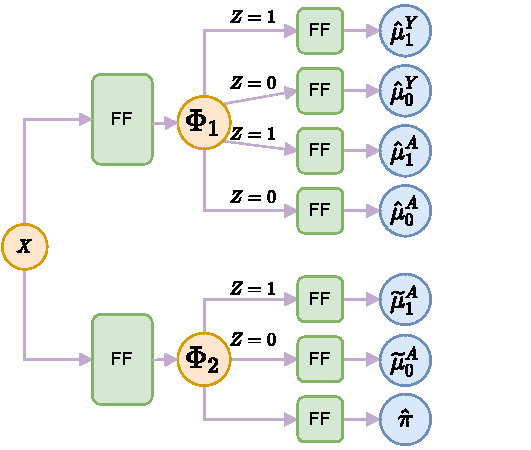
\includegraphics[width=0.4\textwidth]{img/mrnet}
\end{center}
\vspace{-0.5cm}
\caption{Architecture of \modelname.}
\label{fig:mrnet}
\end{wrapfigure}
This ensures that the nuisance estimators (i) share minimal information with nuisance estimators (i) even though they are estimated on the same data.
Intuitively, this should lead to a faster decay of the oracle upper bound (cf. \cite{Curth.2021}). 

%A similar result has been reported for the DR-Learner in combination with TARNet \cite{Curth.2021}.

The architecture of \modelname is shown in Fig.~\ref{fig:mrnet}. \modelname takes the observed covariates $X$ as input to build the two representations $\Phi_1$ and $\Phi_2$. The first representation $\Phi_1$ is used to output estimates $\hat{\mu}_1^Y(x)$, $\hat{\mu}_0^Y(x)$, $\hat{\mu}_1^A(x)$, and $\hat{\mu}_0^A(x)$ of the ITE components. The second representation $\Phi_2$ is used to output estimates $\widetilde{\mu}_1^A(x)$, $\widetilde{\mu}_0^A(x)$, and $\hat{\pi}(x)$. \modelname is trained by minimizing an overall loss
\begin{equation}
\hspace{-0.4cm}
    \mathcal{L}(\theta) = \sum_{i=1}^n \left[ \left(\hat{\mu}_{z_i}^Y(x_i) - y_i \right)^2 + \mathrm{BCE}\left(\hat{\mu}_{z_i}^A(x_i), a_i \right) + \mathrm{BCE}\left(\widetilde{\mu}_{z_i}^A(x_i), a_i \right) +  \mathrm{BCE}\left(\hat{\pi}(x_i), z_i \right) \right],
\end{equation}
where $\theta$ denotes the neural network parameters and $\mathrm{BCE}$ is the binary cross entropy loss. After training \modelname, we obtain the $\hat{\tau}_{\mathrm{init}}(x) = \frac{\hat{\mu}_1^Y(x) - \hat{\mu}_0^Y(x)}{\hat{\mu}_1^A(x) - \hat{\mu}_0^A(x)}$ and perform Stage~1 of \frameworkname to obtain the nuisance estimators $\hat{\mu}_0^Y(x)$, $\hat{\mu}_0^A(x)$, $\hat{\delta}_A(x) = \widetilde{\mu}_1^A(x) - \widetilde{\mu}_0^A(x)$ and $\hat{\pi}(x)$. Then, we perform the Stage~2 pseudo regression of \frameworkname to obtain $\hat{\tau}_{\mathrm{\frameworkname}}(x)$.


\textbf{Implementation:} We use PyTorch Lightning for our implementation and train \modelname with the Adam optimizer \cite{Kingma.2015}. Details  on the network architecture and hyperparameter tuning are in Appendix~\ref*{app:hyper}. We perform both the training of \modelname and the pseudo outcome regression on the full training data. Needless to say, \modelname can be easily adopted for sample splitting or cross-fitting procedures as in \cite{Chernozhukov.2018}, namely, by learning separate networks for each representation $\Phi_1$ and $\Phi_2$. However, in our experiments, we do not use sample splitting or cross-fitting, as this can affect the performance in finite sample regimes. Of note, our choice is consistent with previous work \cite{Curth.2021}.


\section{Computational experiments}
\label{sec:experiments}

%We perform extensive experiments both on simulated and real-world data to %investigate the performance of \frameworkname and \modelname.

\subsection{Simulated data}

In causal inference literature, it is common practice to use simulated data for performance evaluations \cite{Bica.2020, Curth.2021, Hartford.2017}. Simulated data has the important benefit that it provides ground truth information on the counterfactual outcomes and thus allows direct benchmarking against the oracle ITE.

\textbf{Data generation:}
We generate simulated data by sampling the oracle ITE $\tau(x)$ and the nuisance components $\mu_i^Y(x)$, $\mu_i^A(x)$, and $\pi(x)$ from Gaussian process priors. Using Gaussian processes has the following advantages: (1)~It allows for a fair method comparison, as there is no need to explicitly specify the nuisance components, which could lead to unwanted inductive biases favoring a specific method; (2)~the sampled nuisance components are non-linear and thus resemble scenarios where machine learning methods would be applied; and, (3)~by sampling from the prior induced by the Matern kernel \cite{Rasmussen.2008}, we can control the smoothness of the nuisance components, which allows us to confirm our theoretical results from Sec.~\ref{sec:theory}.

Once we have obtained $\tau(x)$, $\mu_i^Y(x)$, $\mu_i^A(x)$, and $\pi(x)$, we sample $n$ observed confounder $X \sim \mathcal{N}(0,1)$, unobserved confounders $U \sim \mathcal{N}\left(0, 0.2^2\right)$, and instruments $Z \sim \mathrm{Bernoulli}(\pi(X))$. Then, we generate treatments via
\begin{equation}\label{eq:sim_treat}
     A = Z \, \mathbbm{1}\{U + \epsilon_{A} > \alpha_1(X)\} + (1-Z) \, \mathbbm{1}\{U + \epsilon_{A} > \alpha_0(X)\}
\end{equation}
with $\epsilon_{A} \sim \mathcal{N}\left(0, 0.1^2\right)$ and $\alpha_i(X) = \Phi^{-1}\left(1 - \mu_i^A(X)\right) \sqrt{0.1^2 + 0.2^2}$, where $\Phi^{-1}$ denotes the qunatile function of the standard normal distribution. Finally, we generate the outcomes via
{\tiny%
\begin{equation}\label{eq:sim_outcome}
     Y = A \left( \frac{(\mu_1^A(X) - 1)\mu_0^Y(X) - \mu_0^A(X)\mu_1^Y(X) + \mu_1^Y(X)}{\delta_A(X)}\right)+ (1-A) \left( \frac{\mu_1^A(X)\mu_0^Y(X) - \mu_0^A(X)\mu_1^Y(X)}{\delta_A(X)} \right) + \alpha_U U +\epsilon_Y,
\end{equation}}
where $\epsilon_Y \sim \mathcal{N}\left(0, 0.3^2\right)$ and $\alpha_U> 0$ is a parameter indicating the level of unobserved confounding. 
This choice of $A$ and $Y$ in Eq.~\eqref{eq:sim_treat} and Eq.~\eqref{eq:sim_outcome} implies that $\tau(x)$ is indeed the ITE, \ie, it holds that $\tau(x) = \E[Y(1) -Y(0) \mid X = x]$. For a derivation, we refer to Appendix~\ref*{app:sim}.

\textbf{Baselines:}
We compare our \modelname with the following state-of-the-art baselines: (1)~ITE methods for unconfoundedness, i.e., \textbf{TARNet} \cite{Shalit.2017} and TARNet combined with the \textbf{DR learner} \cite{Kennedy.2020}; (2)~general IV methods, i.e., \textbf{2SLS} \cite{Wright.1928}, \textbf{DeepIV} \cite{Hartford.2017}, kernel IV (\textbf{KIV}) \cite{Singh.2019}, \textbf{DeepGMM} \cite{Bennett.2019}, Deep Feature Instrumental Variable Regression (\textbf{DFIV}) \cite{Xu.2021}, \textbf{DMLIV} \cite{Syrgkanis.2019}, and DMLIV combined with \textbf{DRIV} (as described in \cite{Syrgkanis.2019}); (3)~the (plug-in) Wald estimator using \textbf{linear models} and Bayesian additive regression trees (\textbf{BART}) \cite{Chipman.2010}. Of note, the DR learner assumes unconfoundedness, which is why we only combine it TARNet in our experiments. Implementation details regarding baselines and nuisance parameter estimation are in Appendix~\ref*{app:baseline}. 

\TODO{das später in die Results bzs. sensitivty} We also compare \frameworkname and DRIV with different base methods. The nuisance parameters are estimated using feed forward neural networks (DRIV) or TARNets with either binary or continuous outputs (MRIV).

\textbf{Performance evaluation:} For all experiments, we split the data in a training set (80\%) and a test set (20\%). After training, we calculate the root mean squared errors (RMSE) between the ITE estimates and the oracle ITE on the test set. We report the mean RMSE and the standard deviation over five data sets generated from random seeds.

\textbf{Results:}
Table~\ref{tab:base} shows the results for all baselines. Here, the DR learner does not improve the performance of TARNet, which is reasonable as both the DR learner and TARNet assume unconfoundedness and are thus biased in our setting. Our \modelname outperforms all baselines. Our \modelname also achieves a smaller standard deviation. This demonstrates that our \modelname is superior.

\begin{table}[tbp]
\caption{Performance comparison: our \modelname vs. existing baselines.}
\label{tab:base}
\centering
\vspace{-0.3cm}
\label{t:results_sim}
\scriptsize
\begin{tabular}{lccc}
\toprule
{Method} & {$n = 3000$} & {$n = 5000$} & {$n = 8000$} \\
\midrule
\textsc{(1) Standard ITE} & &  & \\
\quad TARNet \cite{Shalit.2017} &$0.76 \pm 0.14$& $0.70 \pm 0.12$ & $0.69 \pm 0.17$\\
\quad TARNet + DR \cite{Shalit.2017, Kennedy.2020} &$0.78 \pm 0.10$& $0.66 \pm 0.09$ & $0.70 \pm 0.10$\\
\midrule
\textsc{(2) General IV} & &  & \\
\quad 2SLS \cite{Wooldridge.2013}&$1.22 \pm 0.23$ &$0.79 \pm 0.37$  & $1.12 \pm 0.29$ \\
\quad DeepIV \cite{Hartford.2017}&$0.96 \pm 0.30$ & $0.28 \pm 0.09$ & $0.23 \pm 0.04$\\
\quad KIV \cite{Singh.2019}&$1.54 \pm 0.53$ & $1.18 \pm 1.14$ &  $3.80 \pm 4.71$\\
\quad DeepGMM \cite{Bennett.2019}&$0.95 \pm 0.38$ &$0.37 \pm 0.09$  & $0.42 \pm 0.14$ \\
\quad DFIV \cite{Xu.2021}&$0.43 \pm 0.11$ & $0.40 \pm 0.21$ & $0.46 \pm 0.54$ \\
\quad DMLIV \cite{Syrgkanis.2019}&$1.92 \pm 0.71$ & $0.92 \pm 0.41$ &  $1.14 \pm 0.24$\\
\quad DMLIV + DRIV \cite{Syrgkanis.2019}&$0.41 \pm 0.12$ & $0.22 \pm 0.04$ &  $0.21 \pm 0.06$\\
\midrule
\textsc{(3) Wald estimator \cite{Wald.1940}} & &  & \\
\quad Linear &$1.06 \pm 0.63$ & $0.62 \pm 0.22$ &  $0.81 \pm 0.34$\\
\quad BART &$0.95 \pm 0.30$ &$0.63 \pm 0.33$ &$0.88 \pm 0.28$\\ \bottomrule \noalign{\smallskip}
\modelname (ours) &$\boldsymbol{0.26 \pm 0.11}$ & $\boldsymbol{0.15 \pm 0.03}$ & $\boldsymbol{0.13 \pm 0.03}$\\

\bottomrule
\multicolumn{4}{l}{Reported: RMSE for base methods (mean $\pm$ standard deviation). Lower $=$ better (best in bold)}
\end{tabular}
\vspace{-0.3cm}
\end{table}

We further compare the performance of two different meta-learner frameworks -- DRIV \cite{Syrgkanis.2019} and our \frameworkname -- across different base methods. The results are in Table~\ref{tab:frameworks}. Our \frameworkname improves over the variant without any meta-learner framework across all base methods (both in terms of RMSE and standard deviation). Furthermore, \frameworkname is clearly superior over DRIV. This demonstrates the effectiveness of our \frameworkname across different base methods (note: \frameworkname with an arbitrary base model is typically superior to DRIV with our custom network from above). \modelname is overall best.

\begin{table}[tbp]
\caption{Base model with different meta-learners (i.e., none, DRIV, and our \frameworkname).}
\label{tab:frameworks}
\centering
\vspace{-0.3cm}
\label{t:results_sim}
\resizebox{\columnwidth}{!}{%
\begin{tabular}{lccccccccc}
\noalign{\smallskip} \toprule \noalign{\smallskip}
& \multicolumn{3}{c}{$n = 3000$} & \multicolumn{3}{c}{$n = 5000$} & \multicolumn{3}{c}{$n = 8000$} \\
\cmidrule(lr){2-4} \cmidrule(lr){5-7} \cmidrule(lr){8-10}
\backslashbox{Base methods}{Meta-learners} & None & DRIV & \frameworkname (ours) & None & DRIV & \frameworkname (ours) & None & DRIV & \frameworkname (ours)\\
\midrule
\textsc{(1) Standard ITE} & &  & \\
\quad TARNet \cite{Shalit.2017}& $0.76 \pm 0.14$&$\boldsymbol{0.31 \pm 0.05}$& $0.34 \pm 0.13$ &$0.70 \pm 0.12$ & $\boldsymbol{0.17 \pm 0.06}$ & $\boldsymbol{0.17 \pm 0.05}$ &$0.69 \pm 0.17$ & $0.21 \pm 0.04$ & $\boldsymbol{0.16 \pm 0.04}$\\
\midrule
\textsc{(2) General IV} & &  & \\
\quad 2SLS \cite{Wooldridge.2013}& $1.22 \pm 0.23$& $0.40 \pm 0.11$ &$\boldsymbol{0.31 \pm 0.08}$ &$0.79 \pm 0.37$ & $\boldsymbol{0.17 \pm 0.09}$ & $0.19 \pm 0.05$ & $1.12 \pm 0.29$  & $0.21 \pm 0.05$& $\boldsymbol{0.16 \pm 0.02}$\\
\quad DeepIV \cite{Hartford.2017}&$0.96 \pm 0.30$ & $0.27 \pm 0.03$ & $\boldsymbol{0.26 \pm 0.05}$ & $0.28 \pm 0.09$& $\boldsymbol{0.18 \pm 0.08}$ & $\boldsymbol{0.18 \pm 0.05}$ & $0.23 \pm 0.04$ & $0.21 \pm 0.03$ & $\boldsymbol{0.16 \pm 0.03}$\\
\quad KIV \cite{Singh.2019}&$1.54 \pm 0.53$ & $0.40 \pm 0.10$& $\boldsymbol{0.39 \pm 0.11}$ & $1.18 \pm 1.14$&  $0.20 \pm 0.08$ & $\boldsymbol{0.17 \pm 0.06}$ & $3.80 \pm 4.71$& $0.31 \pm 0.18$& $\boldsymbol{0.28 \pm 0.19}$\\
\quad DeepGMM \cite{Bennett.2019}&$0.95 \pm 0.38$ & $0.40 \pm 0.15$& $\boldsymbol{0.36 \pm 0.13}$ &$0.37 \pm 0.09$ & $0.24 \pm 0.12$ & $\boldsymbol{0.16 \pm 0.05}$ &$0.42 \pm 0.14$ & $0.21 \pm 0.03$ & $\boldsymbol{0.17 \pm 0.03}$ \\
\quad DFIV \cite{Xu.2021}&$0.43 \pm 0.11$ &$\boldsymbol{0.26 \pm 0.05}$ & $0.27 \pm 0.07$ &$0.40 \pm 0.21$ & $0.18 \pm 0.09$ & $\boldsymbol{0.16 \pm 0.04}$ &$0.46 \pm 0.54$ & $0.21 \pm 0.06$ & $\boldsymbol{0.18 \pm 0.05}$ \\
\quad DMLIV \cite{Syrgkanis.2019}&$1.92 \pm 0.71$ &$0.41 \pm 0.12$ & $\boldsymbol{0.37 \pm 0.11}$ &$0.92 \pm 0.41$ & $0.22 \pm 0.05$ & $\boldsymbol{0.16 \pm 0.05}$ &$1.14 \pm 0.24$ & $0.21 \pm 0.06$& $\boldsymbol{0.18 \pm 0.05}$\\
\midrule
\textsc{(3) Wald estimator \cite{Wald.1940}}& & & & &  & \\
\quad Linear &$1.06 \pm 0.63$ & $0.42 \pm 0.15$& $\boldsymbol{0.38 \pm 0.14}$ &$0.62 \pm 0.22$ &  $\boldsymbol{0.19 \pm 0.09}$ & $0.25 \pm 0.09$ &$0.81 \pm 0.34$ & $0.19 \pm 0.09$ & $\boldsymbol{0.18 \pm 0.04}$\\
\quad BART &$0.95 \pm 0.30$ &$0.48 \pm 0.14$ & $\boldsymbol{0.46 \pm 0.12}$ &$0.63 \pm 0.33$ & $0.26 \pm 0.13$ & $\boldsymbol{0.20 \pm 0.07}$ &$0.88 \pm 0.28$ & $0.31 \pm 0.08$ & $\boldsymbol{0.29 \pm 0.04}$\\
%\noalign{\smallskip} \bottomrule \noalign{\smallskip}
\midrule
\modelname {\textbackslash}w network only (ours) &$0.39 \pm 0.13$ &$0.35 \pm 0.12$ & $\boldsymbol{0.26 \pm 0.11}$ & $0.31 \pm 0.04$& $0.19 \pm 0.13$ & $\boldsymbol{0.15 \pm 0.03}$ & $0.26 \pm 0.06$& $0.18 \pm 0.08$&  $\boldsymbol{0.13 \pm 0.03}$\\

\bottomrule
\multicolumn{10}{l}{Reported: RMSE (mean $\pm$ standard deviation). Lower $=$ better (best improvement over none meta-learner in bold)}
\end{tabular}%
}
\vspace{-0.3cm}
\end{table}

\textbf{Ablation study:} Table~\ref{tab:ablation} compares different variants of our \modelname. These are: (1)~\frameworkname but network only; (2)~\modelname with a single representation for all nuisance estimators; and (3)~our \modelname from above. We observe that \modelname is best. This justifies our proposed network architecture for \modelname. Hence, combing the result from above, our performance gain must be attributed to both our framework \underline{and} the architecture of our deep neural network. 

\begin{table}[tbp]
\vspace{-0.5cm}
\caption{Ablation study.}
\label{tab:ablation}
\centering
\vspace{-0.3cm}
\label{t:results_sim}
\scriptsize
\begin{tabular}{lccc}
\noalign{\smallskip} \toprule \noalign{\smallskip}
{Method} & {$n = 3000$} & {$n = 5000$} & {$n = 8000$} \\
\midrule
\modelname {\textbackslash}w network only &$0.39 \pm 0.13$ & $0.31 \pm 0.04$ &
$0.26 \pm 0.06$\\
\modelname {\textbackslash}w single repr. &$0.28 \pm 0.12$ & $0.21 \pm 0.04$ &
$0.32 \pm 0.10$\\
\modelname (ours) &$\boldsymbol{0.26 \pm 0.11}$ & $\boldsymbol{0.15 \pm 0.03}$ &
$\boldsymbol{0.13 \pm 0.03}$\\
\bottomrule
\multicolumn{4}{l}{Reported: RMSE (mean $\pm$ standard deviation). Lower $=$ better (best in bold)}
\end{tabular}
\vspace{-0.3cm}
\end{table}

%This result is in line with \cite{Curth.2021} for the DR learner and stresses the importance of either learning separate representations or using sample splitting.
 
\textbf{Robustness checks for unobserved confounding and smoothness:} Here, we demonstrate the importance of handling unobserved confounding (as we do in our \frameworkname framework). For this, Fig.~\ref{fig:plt_confounding} plots the results for our \modelname vs. standard ITE without customization for confounding (i.e. TARNet with and without the DR learner) over over different levels of unobserved confounding. The RMSE of both TARNet variants increase almost linearly with increasing confounding. In contrast, the RMSE of our \modelname only marginally. Even for low confounding regimes, our \modelname performs competitively. 

\begin{figure}[h]
\vspace{-0.3cm}
\centering
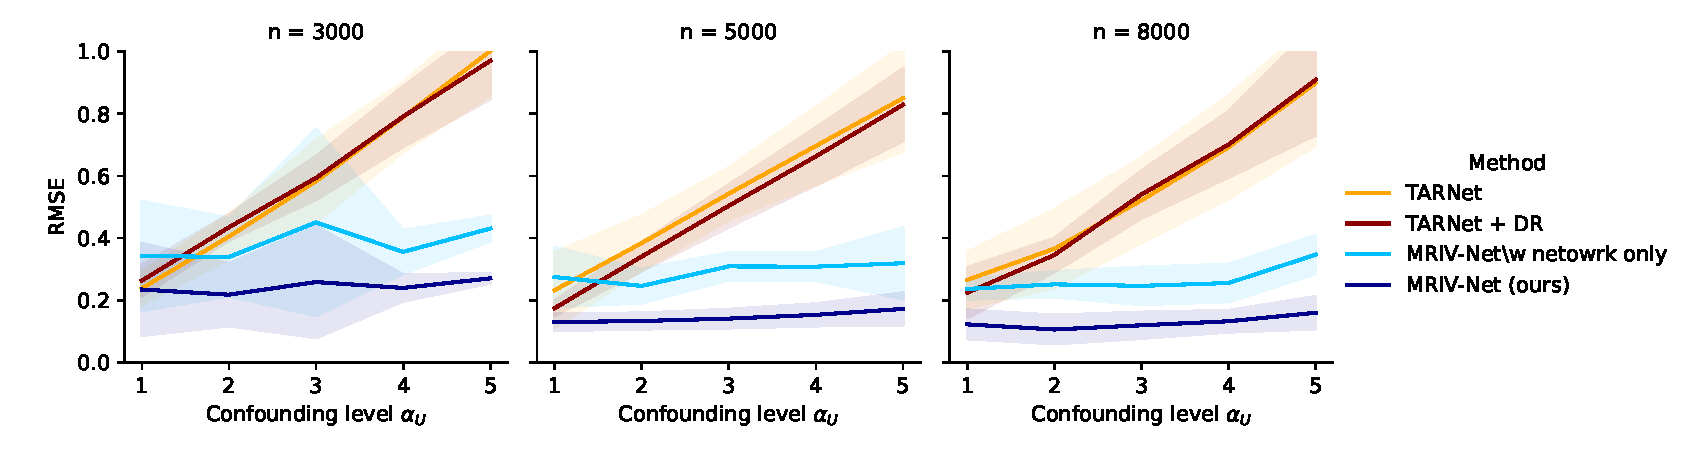
\includegraphics[width=0.8\linewidth]{img/plot_confounding.pdf}
\caption{Results over different levels of confounding $\alpha_U$. Shaded area shows standard deviation.}
\label{fig:plt_confounding}
\vspace{-0.3cm}
\end{figure}

Fig.~\ref{fig:plt_smoothness} varies the smoothness level. This is given by $\alpha$ of $\mu_i^Y(\cdot)$ (controlled by the Matérn kernel prior).
\begin{wrapfigure}{r}{0.5\textwidth}
\vspace{-0.5cm}
 \begin{center}
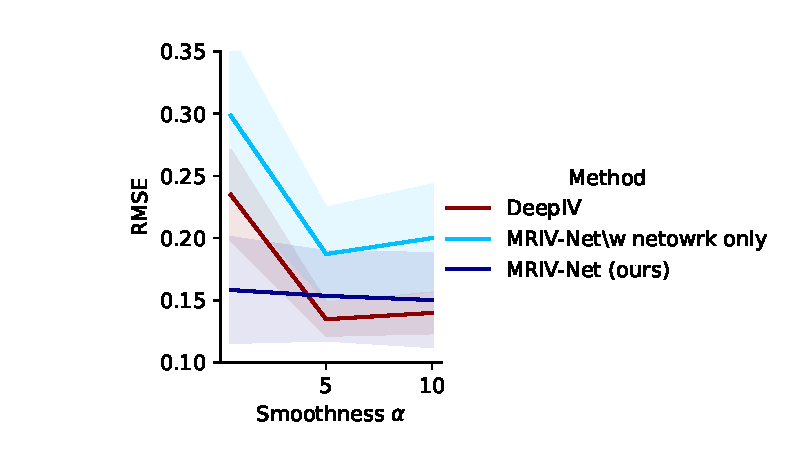
\includegraphics[width=0.5\textwidth]{img/plot_smoothness.pdf}
\end{center}
\vspace{-0.5cm}
\caption{Results over different levels of smoothness $\alpha$  of $\mu_i^Y(\cdot)$, sample size $n=8000$. Larger $\alpha$ = smoother. Shaded areas show standard deviation.}
\vspace{-1.3cm}
\label{fig:plt_smoothness}
\end{wrapfigure}
Here, the performance decreases for the baselines, i.e., DeepIV and our network without \frameworkname framework. In contrast, the peformance of our \modelname remains robust and outperforms the baselines. This thus confirms our theoretical results from above. It thus indicates that our \frameworkname framework works best when the oracle ITE $\tau(x)$ is smoother than the nuisance parameters $\mu_i^Y(x)$.

%We also plot the RMSE of both \modelname versions and DeepIV over the smoothness level $\alpha$ of $\mu_i^Y(\cdot)$ (controlled by the Matern kernel prior). While the performance of both DeepIV and Stage 1 \modelname decreases for low smoothness, \modelname remains stable and outperforms the other mothods. This is in line with our theoretical results, indicating that our \frameworkname framework works best when the oracle ITE $\tau(x)$ is smoother than the nuisance parameters $\mu_i^Y(x)$.
\subsection{Real-world data}\label{sec:exp_real}

\textbf{Setting:} We demonstrate effectiveness of our framework using a case study with real-world, medical data. Here, we use medical data from the so-called \emph{Oregon health insurance experiment} (OHIE) \cite{Finkelstein.2012}. The OHIE data originate from a RCT with non-compliance: In 2008, $\sim$30,000 low-income, uninsured adults in Oregon were offered participation in a health insurance program by a lottery. Individuals whose names were drawn could decide to sign up for health insurance. After a period of 12 months, in-person interviews took place to evaluate the health condition of the respective participant. For our analysis, we treat the lottery assignment as instrument $Z$, the decision to sign up for health insurance as treatment $A$, and an overall health score calculated from the in-person interview questions as outcome $Y$. We also include five observed covariates $X$ including age and gender into our analysis. For details, we refer to Appendix~\ref*{app:real}.

We train our \modelname on a subsample of size 10,000. Then, we estimate the ITE for both genders, fixing the other covariates while varying the age. We repeat the same procedure for our neural network architecture withou the \modelname framework and TARNet. The results are shown in Fig.~\ref{fig:real}.

\textbf{Results:} Our \modelname estimates larger ITEs for an older age. In contrast, TARNet does not estimate positive ITEs even for an older age. 
\begin{wrapfigure}{l}{0.7\textwidth}
\vspace{-0.4cm}
 \begin{center}
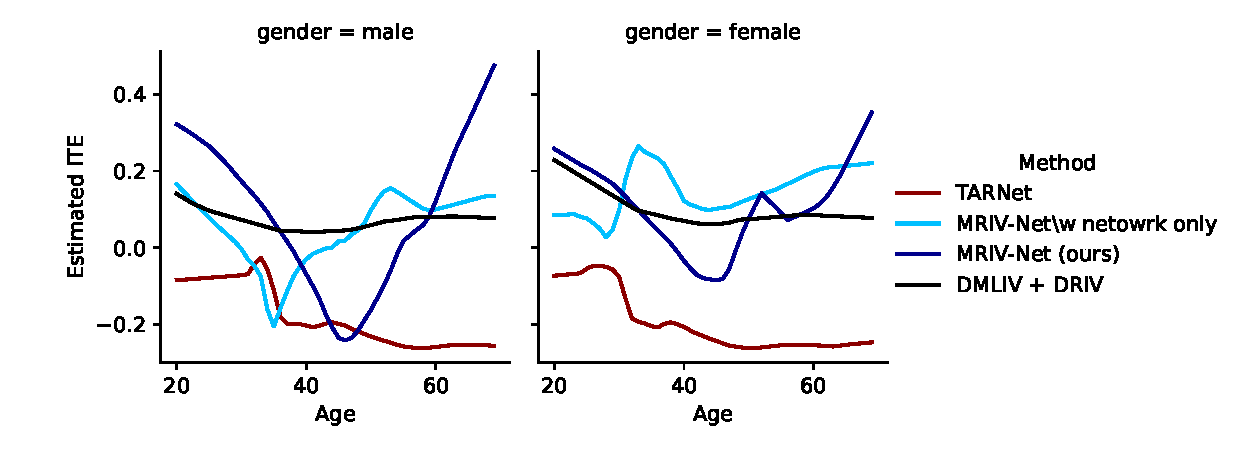
\includegraphics[width=0.7\textwidth]{img/plot_real.pdf}
\end{center}
\vspace{-0.5cm}
\caption{Results on real-world medical data.}
\vspace{-0.7cm}
\label{fig:real}
\end{wrapfigure}
Even though we cannot evaluate the estimation quality on real-world data, our estimates seem reasonable in light of the medical literature: the benefit of health insurance should increase with older age. This showcases that TARNet may suffer from bias induced by unobserved confounders. Interestingly, both our \modelname estimate a somewhat smaller ITE for middle ages (around 30--50 yrs). One explanation might be that individual in this age group are more likely to have stable jobs and, thus, are also more likely to be able to afford medical care, decreasing the direct effect of health insurance on individuals health. In sum, the findings from our case study are of direct relevance for decision-makers in public health \cite{Imbens.1994}, and highlight the practical value of our framework.

\section{Conclusion}
In this paper we propose \modelname, a multiple robust ITE estimator based on a deep neural network. We showed both theoretically and empirically, that \modelname performs competitive and is state-of-the-art of estimating ITEs using binary IVs. For future work, it would be interesting to derive finite sample results for \modelname, because our theoretical analysis is purely asymptotic. Furthermore, one may investigate multiple robust extensions to more general IV settings, i.e., multiple or continuous instruments and treatments.


\begin{ack}
Acknowledgments
\end{ack}

\clearpage
\printbibliography %Prints bibliography



%%%%%%%%%%%%%%%%%%%%%%%%%%%%%%%%%%%%%%%%%%%%%%%%%%%%%%%%%%%%
\section*{Checklist}

\begin{enumerate}


\item For all authors...
\begin{enumerate}
  \item Do the main claims made in the abstract and introduction accurately reflect the paper's contributions and scope?
    \answerYes{See here}
  \item Did you describe the limitations of your work?
    \answerYes{}
  \item Did you discuss any potential negative societal impacts of your work?
    \answerNo{}
  \item Have you read the ethics review guidelines and ensured that your paper conforms to them?
    \answerYes{}
\end{enumerate}


\item If you are including theoretical results...
\begin{enumerate}
  \item Did you state the full set of assumptions of all theoretical results?
    \answerYes{See Sec.~\ref{sec:theory} and Appendix~\ref*{app:proofs}..}
        \item Did you include complete proofs of all theoretical results?
    \answerYes{See Appendix~\ref*{app:proofs}.}
\end{enumerate}


\item If you ran experiments...
\begin{enumerate}
  \item Did you include the code, data, and instructions needed to reproduce the main experimental results (either in the supplemental material or as a URL)?
    \answerYes{(both).}
  \item Did you specify all the training details (e.g., data splits, hyperparameters, how they were chosen)?
    \answerYes{See Appendix~\ref*{app:baseline} and~\ref*{app:hyper}}
        \item Did you report error bars (e.g., with respect to the random seed after running experiments multiple times)?
    \answerYes{One standard deviation using 5 random seeds, see Sec.~\ref{sec:experiments}.}
        \item Did you include the total amount of compute and the type of resources used (e.g., type of GPUs, internal cluster, or cloud provider)?
    \answerYes{See Appendix~\ref*{app:baseline}.}
\end{enumerate}


\item If you are using existing assets (e.g., code, data, models) or curating/releasing new assets...
\begin{enumerate}
  \item If your work uses existing assets, did you cite the creators?
    \answerYes{See Sec.~\ref{sec:exp_real}.}
  \item Did you mention the license of the assets?
    \answerNo{No license is provided on the OHIE website.}
  \item Did you include any new assets either in the supplemental material or as a URL?
    \answerYes{See Appendix~\ref{app:real}.}
  \item Did you discuss whether and how consent was obtained from people whose data you're using/curating?
    \answerNo{We only used simulated and publicly available data.}
  \item Did you discuss whether the data you are using/curating contains personally identifiable information or offensive content?
    \answerNo{The OHIE data is publicly available, personally identifiable information are censored.}
\end{enumerate}


\item If you used crowdsourcing or conducted research with human subjects...
\begin{enumerate}
  \item Did you include the full text of instructions given to participants and screenshots, if applicable?
    \answerNo{Not applicable.}
  \item Did you describe any potential participant risks, with links to Institutional Review Board (IRB) approvals, if applicable?
    \answerNo{Not applicable.}
  \item Did you include the estimated hourly wage paid to participants and the total amount spent on participant compensation?
    \answerNo{Not applicable.}
\end{enumerate}


\end{enumerate}


%%%%%%%%%%%%%%%%%%%%%%%%%%%%%%%%%%%%%%%%%%%%%%%%%%%%%%%%%%%%
\clearpage
\title{Estimating individual treatment effects under unobserved confounding using binary instruments Appendix}
\maketitle

\appendix

The appendix is organized as follows:

\section{Proofs}\label{app:proofs}

\subsection{Proof of Theorem~\ref{thrm:upperbound}}
Before we prove the Theorem, we derive an explicit expression for $\E[\hat{Y}_0 \mid X=x]$.
\begin{lemma}\label{lem:second_stage}
\begin{equation}
\begin{split}
    \E[\hat{Y}_0 \mid X=x] &= 
   \frac{\pi(x)}{\hat{\delta}_A(x) \hat{\pi}(x)} \left(\mu_1^Y(x) - \mu_1^A(x)\hat{\tau}(x)\right)
   + \frac{(1-\pi(x))}{\hat{\delta}_A(x)(1 - \hat{\pi}(x))} \left(\mu_0^A(x) \hat{\tau}(x) -\mu_0^Y(x) \right)\\ & \quad + 
   \frac{\hat{\mu}_0^A(x) \hat{\tau}(x) - \hat{\mu}_0^Y (x)}{\hat{\delta}_A(x)} \left(\frac{\pi(x)}{\hat{\pi}(x)} - \frac{1- \pi(x)}{1-\hat{\pi}(x)} \right) + \hat{\tau}(x)   
\end{split}
\end{equation}
\end{lemma}

\begin{proof}
\begin{align}
 \E[\hat{Y}_0 \mid X=x] &= \pi(x) \E\left[ \frac{Y - A \hat{\tau}(X) - \hat{\mu}_0^Y(X) + \hat{\mu}_0^A(X) \hat{\tau}(X)}{\hat{\delta}_A(X) \hat{\pi}(X)} \; \middle| \; X = x, Z = 1\right] \\ 
 & \quad + (1 - \pi(x)) \E\left[ \frac{Y - A \hat{\tau}(X) - \hat{\mu}_0^Y(X) + \hat{\mu}_0^A(X) \hat{\tau}(X)}{\hat{\delta}_A(X) (1 - \hat{\pi}(X))} \; \middle| \; X = x, Z = 0\right] + \hat{\tau}(x)\\
 & = \frac{\pi(x)}{\hat{\delta}_A(x) \hat{\pi}(x)} \left( \mu_1^Y(x) - \mu_1^A(x)\hat{\tau}(x) - \hat{\mu}_0^Y(x) + \hat{\mu}_0^A(x)\hat{\tau}(x) \right) \\
 & \quad + \frac{1-\pi(x)}{\hat{\delta}_A(x) (1-\hat{\pi}(x))} \left(\mu_0^Y(x) - \mu_0^A(x)\hat{\tau}(x) - \hat{\mu}_0^Y(x) + \hat{\mu}_0^A(x)\hat{\tau}(x) \right) + \hat{\tau}(x)
\end{align}

Rearranging the terms yields the result.
\end{proof}

\begin{assumption}[Kennedy]
Assumptions from Theorem 1 in \cite{Kennedy.2020}:
\begin{enumerate}
        \item $\hat{\E}_n[W + c \mid X = x] = \hat{\E}_n[W \mid X = x] + c$ for any random $W$ and constant $c$
    \item If $\E[W \mid X = x]$ = $E[V \mid X = x]$ then
    \begin{equation}
        \E\left[\left(\hat{\E}_n[W \mid X = x] - \E[W \mid X = x] \right)^2\right] \asymp \E\left[\left(\hat{\E}_n[V \mid X = x] - \E[V \mid X = x] \right)^2\right].
    \end{equation}
\end{enumerate}
\end{assumption}
\begin{proof}[Proof of Theorem~\ref{thrm:upperbound}]
Applying Theorem~1 of \cite{Kennedy.2020} yields
\begin{equation}
    \E\left[\left(\hat{\tau}(x) - \tau(x)\right)^2\right] \lesssim  \mathcal{R}(x) + \E\left[\hat{r}(x)^2 \right],
\end{equation}
where $\mathcal{R}(x) = \E\left[\left(\widetilde{\tau}_{MR}(x) - \tau(x)\right)^2\right]$ is the oracle risk of the second stage regression and $r(x) = \E[\hat{Y}_0 \mid X = x] - \tau(x)$.
Hence, we can apply Lemma~\ref{lem:second_stage} and get
\begin{align}
   \hat{r}(x) &=  \frac{\pi(x)}{\hat{\delta}_A(x) \hat{\pi}(x)} \left(\mu_1^Y(x) - \mu_1^A(x)\hat{\tau}(x)\right)
   + \frac{(1-\pi(x))}{\hat{\delta}_A(x)(1 - \hat{\pi}(x))} \left(\mu_0^A(x) \hat{\tau}(x) -\mu_0^Y(x) \right)\\ & \quad + 
   \frac{\hat{\mu}_0^A(x) \hat{\tau}(x) - \hat{\mu}_0^Y (x)}{\hat{\delta}_A(x)} \left(\frac{\pi(x)}{\hat{\pi}(x)} - \frac{1- \pi(x)}{1-\hat{\pi}(x)} \right) + \hat{\tau}(x) - \tau(x) \\
   &= \frac{\mu_1^Y(x) - \mu_0^Y(x)}{\hat{\delta}_A(x)} \frac{\pi(x)}{\hat{\pi}(x)} + \frac{\mu_0^Y(x) - \hat{\mu}_0^Y(x)}{\hat{\delta}_A(x)} \left(  \frac{\pi(x)}{\hat{\pi}(x)} -  \frac{1 - \pi(x)}{1 - \hat{\pi}(x)} \right)  + \left(\hat{\tau}(x) - \tau(x)\right)\\
   & \quad + \frac{(\mu_0^A(x) - \mu_1^A(x)) \hat{\tau}(x)}{\hat{\delta}_A(x)} \frac{\pi(x)}{\hat{\pi}(x)} + \frac{(\hat{\mu}_0^D(x) - \mu_0^D(x))\hat{\tau}(x)}{\hat{\delta}_A(x)} \left(  \frac{\pi(x)}{\hat{\pi}(x)} -  \frac{1 - \pi(x)}{1 - \hat{\pi}(x)} \right) \\
   &= \frac{\delta_Y(x) \pi(x)}{\hat{\delta}_A(x) \hat{\pi}(x)} + \frac{\left(\mu_0^Y(x) - \hat{\mu}_0^Y(x)\right) \left(\pi(x) - \hat{\pi}(x)\right)}{\hat{\delta}_A(x) \hat{\pi}(x) \left(1 - \hat{\pi}(x) \right)} + \left(\hat{\tau}(x) - \tau(x)\right) \\
   & \quad - \frac{\delta_A(x) \pi(x) \hat{\tau}(x)}{\hat{\delta}_A(x) \hat{\pi}(x)} + \frac{\left(\hat{\mu}_0^A(x) - \mu_0^A(x)\right) \hat{\tau}(x) \left(\pi(x) - \hat{\pi}(x) \right)}{\hat{\delta}_A(x) \hat{\pi}(x) \left(1 - \hat{\pi}(x)\right)} \\
   &=\frac{\left(\pi(x) - \hat{\pi}(x) \right)}{\hat{\delta}_A(x) \hat{\pi}(x) \left(1 - \hat{\pi}(x)\right)}\left\{\left(\mu_0^Y(x) - \hat{\mu}_0^Y(x)\right) + \left(\hat{\mu}_0^A(x) - \mu_0^A(x)\right)\hat{\tau}(x)\right\} \\
   & \quad + \left(\hat{\tau}(x) - \tau(x)\right) + \frac{\pi(x) \delta_A(x)}{\hat{\pi}(x) \hat{\delta}_A(x)} \left(\tau(x) - \hat{\tau}(x)\right) \\
   &= \frac{\left(\pi(x) - \hat{\pi}(x) \right)}{\hat{\delta}_A(x) \hat{\pi}(x) \left(1 - \hat{\pi}(x)\right)}\left\{\left(\mu_0^Y(x) - \hat{\mu}_0^Y(x)\right) + \left(\hat{\mu}_0^A(x) - \mu_0^A(x)\right)\hat{\tau}(x)\right\} \\
   & \quad + \left(\tau(x) - \hat{\tau}(x)\right) \left(\delta_A(x) - \hat{\delta}_A(x)\right) \pi(x) + \left(\tau(x) - \hat{\tau}(x)\right) \left(\pi(x) - \hat{\pi}(x)\right) \hat{\delta}_A(x).
\end{align}

The inequality $(a+b)^2 \leq 2(a^2 + b^2)$ yields together with $\pi(x) \leq 1$ and the boundedness assumptions
\begin{align}
    \hat{r}(x)^2 & \leq \frac{4}{\epsilon^4 \rho^2} \left(\pi(x) - \hat{\pi}(x) \right)^2 \left\{\left(\mu_0^Y(x) - \hat{\mu}_0^Y(x)\right)^2 + \left(\hat{\mu}_0^A(x) - \mu_0^A(x)\right)^2C^2\right\} \\
    & \quad +4 \left(\tau(x) - \hat{\tau}(x)\right)^2 \left(\delta_A(x) - \hat{\delta}_A(x)\right)^2 + 4\left(\tau(x) - \hat{\tau}(x)\right)^2 \left(\pi(x) - \hat{\pi}(x)\right)^2 
\end{align}

By setting $\widetilde{C} = \max(C,1)$ we obtain
\begin{align}
    \hat{r}(x)^2 & \leq \frac{4\widetilde{C}^2}{\epsilon^4 \rho^2}\left( \left(\pi(x) - \hat{\pi}(x) \right)^2 \left\{\left(\mu_0^Y(x) - \hat{\mu}_0^Y(x)\right)^2 + \left(\hat{\mu}_0^A(x) - \mu_0^A(x)\right)^2 + \left(\hat{\tau}(x) - \tau(x)\right)^2\right\} \right.\\
    & \quad + \left. \left(\tau(x) - \hat{\tau}(x)\right)^2 \left(\delta_A(x) - \hat{\delta}_A(x)\right)^2 \right).
\end{align}

Applying expectations on both sides yields

\begin{equation}
\begin{split}
    \E\left[\left(\hat{\tau}_{MR}(x) - \tau(x)\right)^2\right] & \lesssim \mathcal{R}(x)  + \E\left[\left(\hat{\tau}(x) - \tau(x)\right)^2\right] \E\left[\left(\hat{\delta}_A(x) - \delta_A(x)\right)^2\right]
    \\ & \quad + \E\left[\left(\hat{\pi}(x) - \pi(x)\right)^2\right] \left(\E\left[\left(\hat{\mu}_0^Y(x) - \mu_0^Y(x)\right)^2\right] 
     + \E\left[\left(\hat{\mu}_0^A(x) - \mu_0^A(x)\right)^2\right] + \E\left[\left(\hat{\tau}(x) - \tau(x)\right)^2\right] \right),
\end{split}
\end{equation}
becuase $(\hat{\pi}(x), \hat{\delta}_A(x)) \indep (\hat{\mu}_0^Y(x), \hat{\mu}_0^A(x), \hat{\tau}(x))$ due to sample splitting.
The claim follows now from the smoothness assumptions.
\end{proof}

\subsection{Proof of Theorem~\ref{thrm:rate_wald}}
\begin{proof}
We define $\widetilde{C} = \max(C,1)$ and upper bound
\begin{align}
        (\hat{\tau}_W(x) - \tau(x))^2 &= \left(\frac{(\hat{\mu}_1^Y(x) - \mu_1^Y(x)) \delta_A(x) + (\mu_0^Y(x) - \hat{\mu}_0^Y(x))\delta_A(x) + (\delta_A(x) - \hat{\delta}_A(x))\delta_Y(x)}{\delta_A(x)\hat{\delta}_A(x)}\right)^2 \\
        &  \leq \frac{4 \widetilde{C}^2}{\rho^2 \widetilde{\rho}^2} \left\{(\hat{\mu}_1^Y(x) - \mu_1^Y(x))^2 + (\hat{\mu}_0^Y(x) - \mu_0^Y(x))^2 + (\delta_A(x) - \hat{\delta}_A(x))^2 \right\}\\
        &  \leq \frac{8 \widetilde{C}^2}{\rho^2 \widetilde{\rho}^2} \left\{(\hat{\mu}_1^Y(x) - \mu_1^Y(x))^2 + (\hat{\mu}_0^Y(x) - \mu_0^Y(x))^2 + (\hat{\mu}_1^A(x) - \mu_1^A(x))^2 + (\hat{\mu}_0^A(x) - \mu_0^A(x))^2 \right\},
\end{align}
where we used the inequality $(a+b)^2 \leq 2(a^2 + b^2)$ several times.
Taking expectations and applying the smoothness assumptions yields the result.
\end{proof}

\subsection{Proof of Theorem~\ref{thrm:robustness} (multiple robustness property)}

\begin{proof}
We use Lemma~\ref{lem:second_stage} to show that under each of the three conditions it follows that  $\E[\hat{Y}_0 \mid X=x] = \tau(x)$.
\begin{enumerate}
    \item \begin{align}
    \E[\hat{Y}_0 \mid X=x] &=  \frac{\pi(x)}{\delta_A(x) \hat{\pi}(x)} \left(\mu_1^Y(x) - \mu_1^A(x)\tau(x) + \mu_0^A(x) \tau(x) - \mu_0^Y (x)\right) \\
   & \quad + \frac{(1-\pi(x))}{\delta_A(x)(1 - \hat{\pi}(x))} \left(\mu_0^A(x) \tau(x) -\mu_0^Y(x)  - \mu_0^A(x) \tau(x) + \mu_0^Y (x)\right)
    + \tau(x) \\
    &= \frac{\pi(x)}{\delta_A(x) \hat{\pi}(x)} \left(\delta_Y(x) - \delta_Y(x) \right) + \tau(x) = \tau(x)
    \end{align}
    
    \item $\E[\hat{Y}_0 \mid X=x] = \frac{\left(\mu_1^Y(x) - \mu_1^A(x) \hat{\tau}(x)\right)}{\delta_A(x)}
   + \frac{\left(\mu_0^A(x) \hat{\tau}(x) -\mu_0^Y(x) \right)}{\delta_A(x)} + \hat{\tau}(x) = \frac{\delta_Y(x) - \hat{\tau}(x) \delta_A(x)}{\delta_A(x)} + \hat{\tau}(x) = \tau(x)$
  
     \item $\E[\hat{Y}_0 \mid X=x] = \frac{\left(\mu_1^Y(x) - \mu_1^A(x) \tau(x)\right)}{\hat{\delta}_A(x)}
   + \frac{\left(\mu_0^A(x) \tau(x) -\mu_0^Y(x) \right)}{\hat{\delta}_A(x)} + \tau(x) = \frac{\delta_Y(x)}{\hat{\delta}_A(x)} - \tau(x) \frac{\delta_A(x)}{\hat{\delta}_A(x)} + \tau(x) = \tau(x)$.
\end{enumerate}
\end{proof}

\clearpage
\section{Theoretical analysis under sparsity assumptions}\label{app:sparsity}

\clearpage
\section{Simulated data}\label{app:sim}
We simulate the ITE surfaces from Gaussian processes as this allows us to control the smoothness of the different components. More precisely, we use the Matern kernel
\begin{equation}
    K_{\ell, \nu}(x_i, x_j) = \frac{1}{\Gamma(\nu)2^{\nu-1}}\left( \frac{\sqrt{2\nu}}{\ell} \| x_i - x_j\|_2  \right)^\nu K_\nu \left(\frac{\sqrt{2\nu}}{\ell} \| x_i - x_j\|_2 \right),
\end{equation}
where $\Gamma(\cdot)$ is the Gamma function and $K_\nu(\cdot)$ is the modified Bessel function of second kind. Here, $\ell$ is the length scale of the kernel and $\nu$ controls the smoothness of the sampled functions. We sample functions $\tau \sim \mathcal{GP}(0, K_{\ell, \nu_1})$, $c_0 \sim \mathcal{GP}(0, K_{\ell, \nu_2})$, $f_1 \sim \mathcal{GP}(0, K_{\ell, \nu_3})$, $f_0 \sim \mathcal{GP}(0, K_{\ell, \nu_4})$ and $g \sim \mathcal{GP}(0, K_{\ell, \nu_5})$. 
Then, we define $c_1= \tau + c_0$, $\mu_1^A = \widetilde{\sigma} \circ f_1$, $\mu_0^A = \widetilde{\sigma} \circ f_0$, $\delta_A = \mu_1^A - \mu_0^A$, $\mu_1^Y = c_1 \delta_A$, $\mu_0^Y = c_0 \delta_A$, and $\pi = \sigma \circ g$, where $\widetilde{\sigma}(\cdot) = \sigma_U \sigma(\cdot) + (1-\sigma_U)/2$. By construction, we have $\tau = \frac{\mu_1^Y - \mu_0^Y}{\mu_1^A - \mu_0^A}$.

We sample $n$ observed confounders $X \sim \mathcal{N}_p(0,I)$ and unobserved confounders $U \sim \mathcal{N}\left(0, \sigma_Usi^2\right)$ with $\sigma_U > 0$. Then, we generate treatment assignments
 \begin{equation}
     Z \sim \mathrm{Bernoulli}(\pi(X))
 \end{equation}
 
\begin{equation}
     A = Z \mathbbm{1}\{U + \epsilon_{A} > \alpha_1(X)\} + (1-Z) \mathbbm{1}\{U + \epsilon_{A} > \alpha_0(X)\}
\end{equation}
with $\epsilon_{A} \sim \mathcal{N}\left(0, \sigma_A^2\right)$ and $\alpha_i(X) = \Phi^{-1}\left(1 - \mu_i^A(X)\right) \sqrt{\sigma_A^2 + \sigma_U^2}$.
\begin{equation}
     Y = A \left( \frac{(\mu_1^A(X) - 1)\mu_0^Y(X) - \mu_0^A(X)\mu_1^Y(X) + \mu_1^Y(X)}{\delta_A(X)}\right)+ (1-A) \left( \frac{\mu_1^A(X)\mu_0^Y(X) - \mu_0^A(X)\mu_1^Y(X)}{\delta_A(X)} \right) + \alpha_U U +\epsilon_Y
\end{equation}
 
This choice of $A$ and $Y$ implies that $\tau(x)$ is indeed the ITE curve, \ie,
\begin{equation}
    \tau(x) = \E[Y(1) -Y(0) \mid X = x].
\end{equation}


\clearpage
\section{Oregon health insurance experiment}\label{app:real}
% , which is available online for public use \footnote{Data available here: https://www.nber.org/programs-projects/projects-and-centers/oregon-health-insurance-experiment}

\clearpage
\section{Baseline models}\label{app:baseline}

\clearpage
\section{Hyperparameter tuning}\label{app:hyper}


\end{document}